\section{Fourier Transformation}
\subsection{DFT, FFT}
\begin{frame}{\insertsection}
	\framesubtitle{\insertsubsection}
	
	\begin{figure}
		\includegraphics[width=\linewidth]{images/rectFilter\_impulseresponse.png}
		\caption*{Schaltplan Spannungsbereinigung}
	\end{figure}

\end{frame}


\subsection{Performance}
\begin{frame}{\insertsection}
	\framesubtitle{\insertsubsection}

	\begin{columns}[T] % align columns{\tiny }
	\begin{column}{0.48\textwidth}
		\begin{figure}
			\includegraphics[width=\textwidth, height=0.5\textheight]{images/rectFilter\_impulseresponse.png}
			\caption*{Messung und Bereinigung}
		\end{figure}
	\end{column}
	\hfill
	\begin{column}{0.48\textwidth}
		\begin{figure}
			\includegraphics[width=\textwidth, height=0.5\textheight]{images/rectFilter\_impulseresponse.png}
			\caption*{Timer Interrupt}
		\end{figure}
	\end{column}
	\end{columns}
\end{frame}


\subsection{IDFT}
\begin{frame}{\insertsection}
	\framesubtitle{\insertsubsection}
	
	\begin{itemize}
		\item DFT als Matrix, IDFT als Matrix unitäre Matrix, Normalisierungfaktor
	\end{itemize}
\end{frame}


\subsection{Konvergenzverhalten, Fehleranalyse}
\begin{frame}{\insertsection}
	\framesubtitle{\insertsubsection}
	
	\begin{itemize}
		\item Vandermonde-Matrix
	\end{itemize}
\end{frame}

\subsection{Leck-Effekt, Fensterfunktionen}
\begin{frame}{\insertsection}
	\framesubtitle{\insertsubsection}
	
	\begin{itemize}
		\item Anzahl der Datenpunkte eines zeitdiskreten Signals ist kein ganzzahliges Vielfaches der Periodendauer
		% sehr wahrscheinlich dass der Fall eintritt
		\item DFT gibt Frequenzanteile an, die im unendlich langen Signal nicht vorkämen
		\item Leck-Effekt (spectral leakage) tritt auf, weil das Signal nur endlich lange beobachtet werden kann
	\end{itemize}
	
	\begin{columns}[T] % align columns{\tiny }
		\begin{column}{0.48\textwidth}
			\begin{figure}
				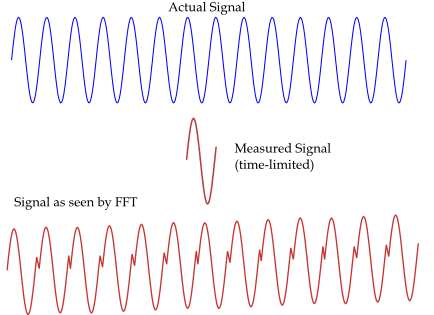
\includegraphics[scale=0.25]{images/spectralLeakage.png}
				\caption*{\centering Zustandekommen des Leck-Effekts, \href{https://www.gaussianwaves.com/2011/01/fft-and-spectral-leakage-2/}{\tiny https://www.gaussianwaves.com/2011/01/fft-and-spectral-leakage-2/}}
			\end{figure}
		\end{column}
		\hfill
		\begin{column}{0.5\textwidth}
			\begin{figure}
				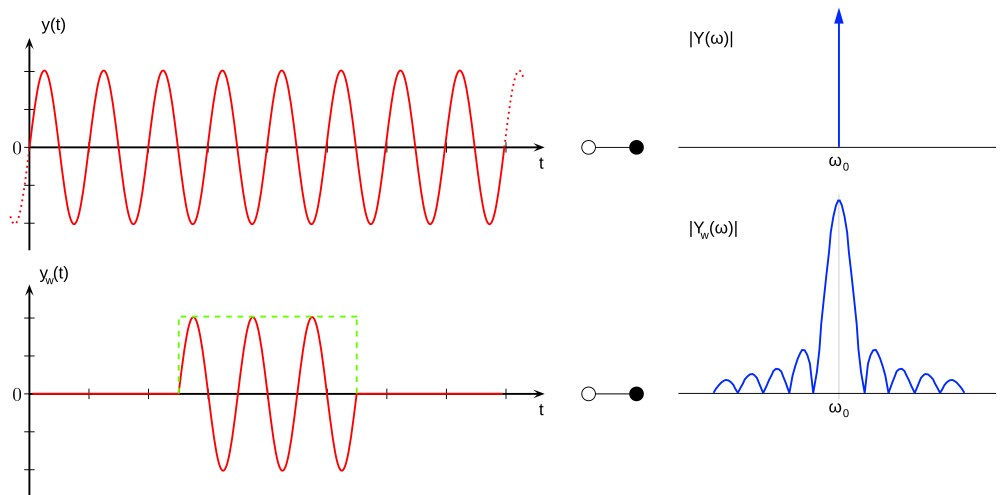
\includegraphics[scale=0.185]{images/spectralLeakage-WindowFunction.png}
				\caption*{\centering implizite Anwendung eines Rechteck-Fensters, \href{https://de.wikipedia.org/wiki/Leck-Effekt}{\tiny https://de.wikipedia.org/wiki/Leck-Effekt}}
			\end{figure}
		\end{column}
	\end{columns}
\end{frame}

\begin{frame}{\insertsection}
	\framesubtitle{\insertsubsection}
	
	\begin{itemize}
		\item Leck-Effekt lässt sich nicht komplett vermeiden
		\item Auswirkung aber reduzierbar durch Fensterfunktionen
		\item Fensterfunktion wird vor der DFT Operation auf das Signal angewendet, sodass das Signal
				  künstlich periodisiert wird
				  % wenn man kein Fenster verwendet wird implizit das Rechteck-Fenster (Daten*1) angewendet,
				  % weil die Daten nur endlich lang sind
				  % Faltungssatz: Multiplikation im Zeitbereich ist Faltung der Fourier Transformierten und andersherum
				  % => Frequenzspektrum ist die Faltung aus DFT(Daten), DFT(Rechteck)
				  % wobei DFT(Rechteck) die Sinc-Funktion ist und diese hat Ripples
		\begin{figure}
			\centering
			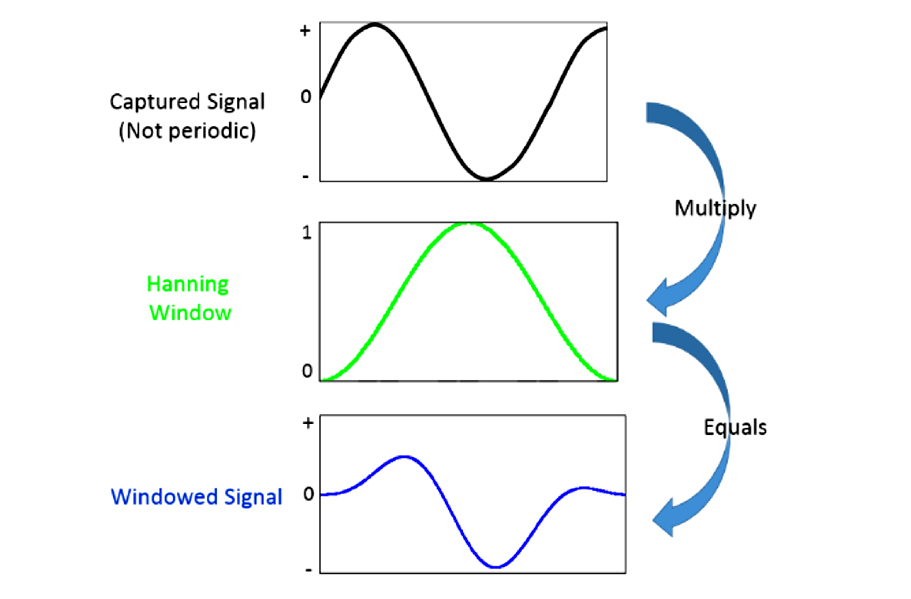
\includegraphics[scale=0.4]{images/appliedWindowFunction2.jpg}
			\caption*{\centering Anwendung des Von-Hann-Fensters,\\ \href{https://www.modalshop.com/rental/learn/basics/how-to-choose-fft-window}{\tiny https://www.modalshop.com/rental/learn/basics/how-to-choose-fft-window}}
		\end{figure}
	\end{itemize}
\end{frame}














 